\beginsong{Wenn die Zeit gekommen ist}[wuw={mac (Erik Martin)}, pfii={100}, pfiii={8}]

\beginverse
\endverse
\centering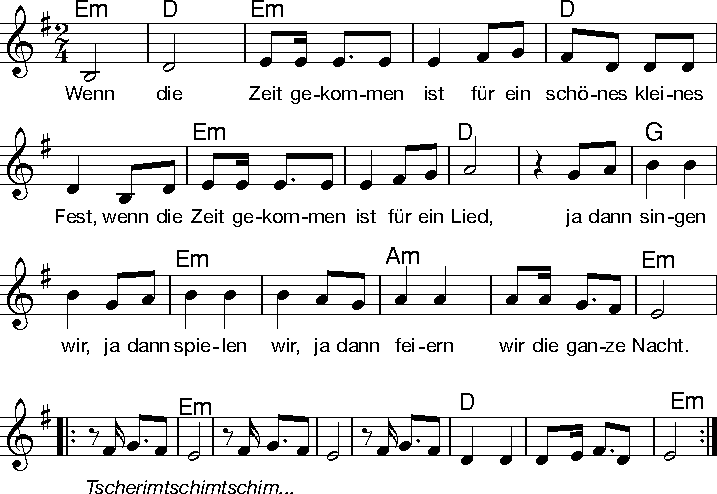
\includegraphics[width=1\textwidth]{Noten/Lied097.pdf}

\beginverse
\[Em]Wenn \[D]die \[Em]Zeit gekommen ist für ein \[D]herrliches Getränk,
wenn die \[Em]Zeit gekommen ist für den \[D]Tschai,
ja dann \[G]kochen wir, ja dann \[Em]feiern wir,
ja dann \[Am]trinken wir die ganze \[Em]Nacht.
\endverse

\beginchorus
\lrep Tscherimtschim\[Em]tschim tscherimtschimtschim,
 tscherimtschim\[D]tschimtschim tscherim\[Em]tschimtschim \rrep
\endchorus 

\beginverse
^Wenn ^die ^Zeit gekommen ist, an die ^Arbeit dann zu geh'n,
wenn die ^Zeit gekommen ist für die ^Tat,
ja dann ^bauen wir, ja dann ^werken wir,
ja dann ^schaffen wir den ganzen ^Tag.
\endverse
%\renewcommand{\everychorus}{\textnote{\bf Refrain (wdh.)}}

\beginchorus
\lrep Tscherimtschim\[Em]tschim tscherimtschimtschim,
 tscherimtschim\[D]tschimtschim tscherim\[Em]tschimtschim \rrep
\endchorus 

\endsong
